\documentclass{beamer}

% For more themes, color themes and font themes, see:
% http://deic.uab.es/~iblanes/beamer_gallery/index_by_theme.html
%
\mode<presentation>
{
% Madrid is a good basic theme
%good themes: Antibes/dolphin, Boadilla/beaver/crane

  \usetheme{Antibes}       % or try default, Darmstadt, Warsaw, ... I like Singapore, 
  \usecolortheme{dolphin} % or try albatross, beaver, crane, ... I like seahorse, crane, or beaver
  \usefonttheme{serif}    % or try default, structurebold, ...
  \setbeamertemplate{navigation symbols}{}
  \setbeamertemplate{caption}[numbered]
  \setbeamertemplate{bibliography item}[text]
} 
\usepackage[english]{babel}
\usepackage[utf8x]{inputenc}
\usepackage{pgfpages}
\pgfpagesuselayout{resize to}[%
  physical paper width=8in, physical paper height=6in]


% Pacakges and commands that I like:
%For math symbols
\usepackage{amsmath} 
\usepackage{amsfonts}%
\usepackage{amssymb}
\usepackage{amsthm}
%\usepackage{titlesec}
%For Graphics
\usepackage{graphicx}
\usepackage{multicol}
\usepackage{subcaption}
%Setup Page
%\usepackage{fullpage} 
% \usepackage[margin=.5in]{geometry}
% \usepackage{fancyhdr}
% \pagestyle{fancy}
% \setlength{\headheight}{14pt}

\def \R{\ensuremath \mathbb{R}}
\def \e{\ensuremath \varepsilon}
\def \d{\ensuremath \delta}
\def \tr{\ensuremath \text{tr}}
\newcommand{\vect}[1]{\boldsymbol{#1}}
\theoremstyle{definition}
\newtheorem{defn}{Definition}[section]
\newtheorem{thm}{Theorem}[section]
\newtheorem*{cor}{Corollary}


%%%%%%%%%%%%%%%%%%%%%%%%%%%%%%%%%%%%%%%%%%%%%%%%%%%%%%%%%%%%%%%%%%%%%%%%%%%%%%
%%%%%%%%%%%%%%%%%%%%%%%%%%%%%%%%%%%%%%%%%%%%%%%%%%%%%%%%%%%%%%%%%%%%%%%%%%%%%%
% Here's where the presentation starts, with the info for the title slide
\title[Knowledge Tracing]{An Introduction to Knowledge Tracing}
\author{Geoffrey Converse}
\institute{University of Iowa}
\date{February 4, 2021}

\begin{document}


\begin{frame}
  \titlepage
\end{frame}


\begin{frame}{Outline}
  \tableofcontents
\end{frame}

\section{Overview}

\begin{frame}{High-level view}
  \begin{itemize}
    \item Given a sequence of responses to an (online) assessment
    \item Each exercise is associated with a latent concept
    \item How does the student's mastery of each concept progress throughout the exam?
    \item Applications include feedback evaluation, intelligent tutoring systems
  \end{itemize}
\end{frame}


\section{Mathematical Setup}

\begin{frame}{Notation}
  \begin{itemize}
    \item $N$ students, indexed by $j$
    \item $n$ available items, indexed by $i$
    \item $K$ concepts, indexed by $k$
    \item $L$ maximum length response sequence, each timestep indexed by $t$
      \begin{itemize}
        \item If a student answers $<L$ questions, then pad their sequence
        \item If a student answers $>L$ questions, then split into two sequences
      \end{itemize}
    \item Interactions are presented as tuple $(q_t, c_t)$ 
      \begin{itemize}
        \item $q_t$ is an integer $\leq n$ that indexes an item
        \item $c_t \in \{0,1\}$ indicates correct/incorrect
        \item $2n$ possible interactions -- can one-hot encode $(q_t,c_t)$
      \end{itemize}
  \end{itemize}
\end{frame}

\begin{frame}{Data Example}
\begin{itemize}
  \item Set $L = 4$, $n=6$
  \item Student $a$ answers questions $\{1,4,2\}$
    \begin{itemize}
      \item $X_a = \{(PAD, PAD), (1,0), (4,1), (2,1)\}$
    \end{itemize}
  \item Student $b$ answers questions $\{2,5,3,1,6\}$
    \begin{itemize}
      \item $X_{b_1} = \{(PAD, PAD), (2,0), (5,1), (3,1)\}$
      \item $X_{b_2} = \{(PAD, PAD), (PAD, PAD), (1,0), (6,1)\}$
    \end{itemize}
  \item PAD inputs are ignored
  \item One-hot encode each interaction in vector of length $12$
    \begin{itemize}
      \item $(1,0) \rightarrow v_{10} = [1,0,0,0,0,0,0,0,0,0,0,0]$
      \item $(4,1) \rightarrow v_{41} = [0,0,0,0,0,0,0,1,0,0,0,0]$
    \end{itemize}
  \item Multiply with embedding matrix $A \in \R^{h \times 2n}: \quad \rightarrow x_{10} = Av_{10}$
    \begin{itemize}
      \item Student $a$'s input to neural network: $[PAD, x_{10}, x_{41}, x_{21}]$
    \end{itemize}
\end{itemize}
\end{frame}

\begin{frame}{Goal}
  \begin{itemize}
    \item Given a student's responses $\{(q_1, c_1), \ldots ,(q_t, c_t), (q_{t+1}, ?)\}$, infer $c_{t+1}$ 
    \item Try to approximate \[P(c_{t+1} = 1 | q_1,c_1, \ldots ,q_t, c_t, q_{t+1})\]
    \item[] 
    \item Mask future interactions while training
  \end{itemize}
\end{frame}


\section{Time-series neural networks}
\begin{frame}{Recurrent Neural Networks}
  \begin{multicols}{2}
  
  \begin{itemize}
    \item Input vectors $\vect x_1,\ldots,\vect x_L$
    \item Outputs $\vect y_1, \ldots, \vect y_L$
    \item Hidden states $\vect h_1, \ldots, \vect h_L$
  \end{itemize}
  \begin{align*}
    \vect h_t &= \tanh(W^{hx} \vect x_t + W^{hh} h_{t-1} + b^h)\\
    \vect y_t &= \sigma(W^{yh} \vect h_t + b^y)
  \end{align*}

  \columnbreak
  \begin{center}
  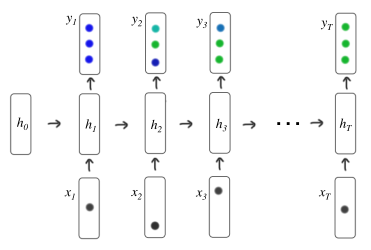
\includegraphics[width=.48\textwidth]{kt_img/rnn.png}
\end{center}
    \\ In knowledge tracing: \\True $y_1$ is given in $x_2$
\end{multicols}
\end{frame}

\begin{frame}{Long Short-Term Memory networks}
  \begin{center}
    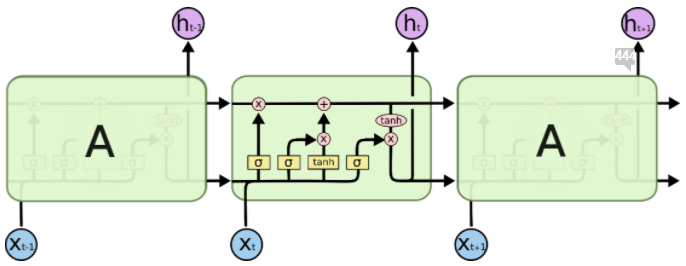
\includegraphics[width=1\textwidth]{kt_img/lstm.png}
  \end{center}
\end{frame}

\begin{frame}{LSTM}
  \begin{itemize}
    \item Forget content: $\vect f_t = \sigma(W_1 [\vect x_t, \vect h_{t-1}] + b_1)$
    \item Input content: $\vect w_t = \sigma(W_2 [\vect x_t,\vect h_{t-1}] + b_2)$ and $\vect a_t = \tanh(W_3 [\vect x_t,\vect h_{t-1}] + b_3)$
    \item Update cell state: $\vect C_t = (\vect f_t \times\vect C_{t-1}) + (\vect w_t \times \vect a_t$) elementwise
      \item Output gate $\vect h_t = \sigma(W_4 [\vect x_t,\vect h_{t-1}] + b_4) \times \tanh(W_5 \vect C_t + b_5)$
  \end{itemize}
\end{frame}


\section{Literature}
\begin{frame}{Deep Knowledge Tracing}
  \begin{itemize}
    \item Really just applied RNN / LSTM to knowledge tracing application
    \item Input $x_t$ is the embedding of $(q_t, c_t)$
    \item Output $y_t$ is the predicted probability that $c_{t+1} = 1$
  \end{itemize}
\end{frame}

\begin{frame}{Dynamic Key-Value Memory Networks}
  \begin{figure}
    \centering
    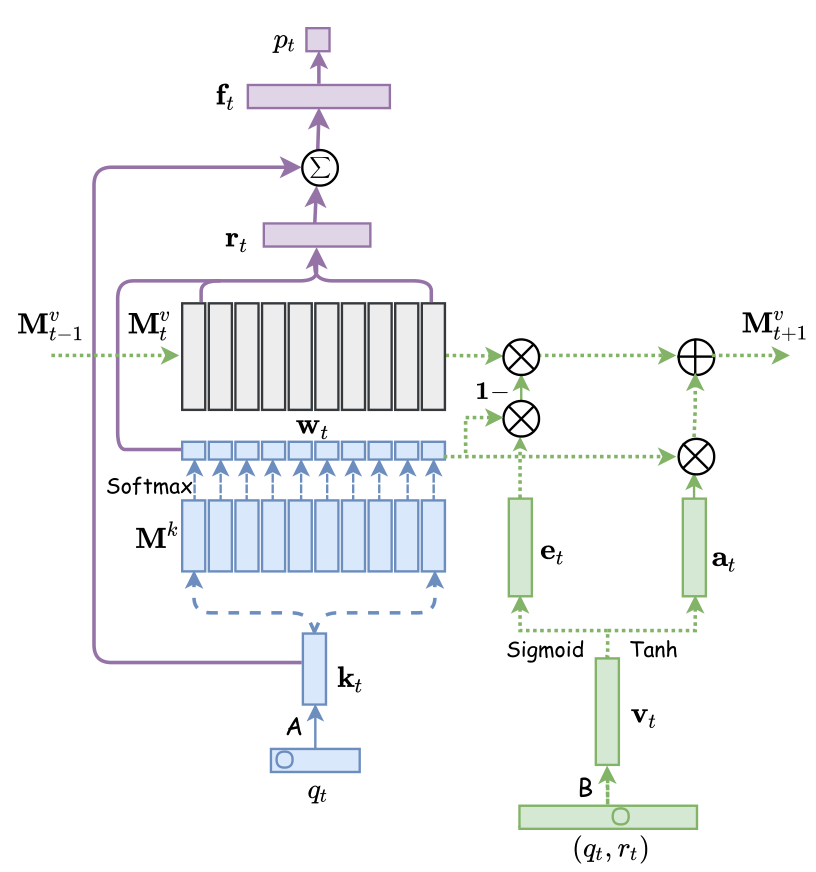
\includegraphics[width=.5\textwidth]{kt_img/dkvmn_arch.png}
    \caption{Architecture of DKVMN}
    \label{fig:dkvmn_arch}
  \end{figure}
\end{frame}

\begin{frame}{DKVMN}
  \begin{itemize}
    \item $K$ concepts (memory slots)
    \item hidden dimension $h$
    \item Stored memory matrix at time $t$: $M_t^v$
    \item Embed question (no response) with $k_t = A\cdot q_t$
    \item Embed question + response with $v_t = B\cdot (q_t,c_t)$
    \item Trainable parameters: $A,B, M^k, W_1, b_1, W_2, b_2, W_e, b_e, W_a, b_a$ 
  \end{itemize}
\end{frame}

\begin{frame}{DKVMN}
READ:
\begin{itemize}
  \item correlation weight $w_t(i) =  \text{Softmax}(k_t^\top M^k(k))$
  \item read content $r_t = \sum_{i=1}^K w_t(i) M^v(i)$
  \item feed forward: $p_t = \sigma(W_2\cdot \left( W_1[r_t, k_t] + b_1 \right) + b_2)$
\end{itemize}
WRITE:
\begin{itemize}
  \item Erase vector: $e_t = \sigma(W_e v_t + b_e)$
  \item Add vector: $a_t  = \tanh(W_a v_t + b_a)$
  \item Update memory:\[M_t^v(i) = \left( M_{t-1}^v(i) \cdot [1 - w_t(i) e_t] \right) + w_t(i) a_t\]
\end{itemize}
\end{frame}

\begin{frame}{Self-Attentive Knowledge Tracing}
Main mechanism: calculating ``attention''
  \begin{itemize}
    \item For each interaction embedding $x_t$, calculate query, key, and value vectors:
      \[q_t = W^Q x_t, \quad k_t = W^K x_t, \quad v_t = W^V x_t, \quad \text{matrices}\in \R^{h \times h}\]
    \item Calculate the correlation weight between interaction $t$ and all previous exercises:
      \[w_{ti} = \text{Softmax} \left(\frac{q_t^\top k_i}{\sqrt{h}}\right), \quad i \leq t\]
    \item Multiply $w_{ti}$ by correponding value vectors:
      \[A_{ti} = w_{ti} v_i\]
      \[h_t = \sum_{i \leq t} A_{ti}\]
  \end{itemize}
\end{frame}

\begin{frame}{SAKT}
  \begin{figure}
    \centering
    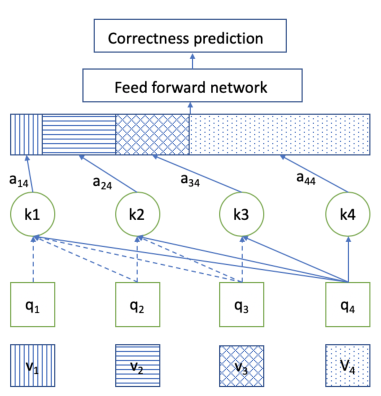
\includegraphics[width=.45\textwidth]{kt_img/sakt_arch.png}
    \caption{SAKT architecture}
    \label{fig:sakt}
  \end{figure}
  $h_t$ is sent through feed forward network to make prediction about next interaction
\end{frame}

\section{New Approaches}

\begin{frame}{IRT-inspired knowledge tracing}
  \begin{figure}
    \centering
    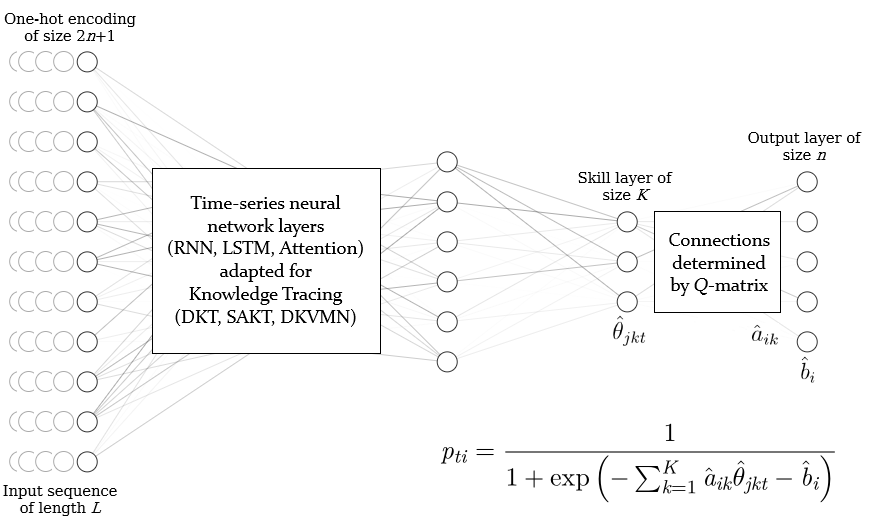
\includegraphics[width=1\textwidth]{kt_img/kt_irt_visual_with_equation.png}
    \caption{Proposed model incorporating IRT with KT}
    \label{fig:kt_irt}
  \end{figure}
\end{frame}
\section{}
\begin{frame}{References}
\begin{thebibliography}{2}
\tiny

\bibitem{bkt} Corbett and Anderson. ``Knowledge Tracing: Modeling the Acquisition of Procedural Knowledge.'' User Modeling and User-Adapted Interaction, 1995. Volume 4, pages 253-278.

\bibitem{dkt} Piech, Bassen, Huang, Ganguli, Shami, Guibas, Shol-Dickstein. ``Deep Knowledge Tracing.'' Advances in Neural Information Processing Systems, 2015.

\bibitem{dkvmn} Zhang, Shi, King, Yeung. ``Dynamic Key-Value Memory Networks for Knowledge Tracing.'' International World Wide Web Conference, 2017. Pages 765-774.

\bibitem{sakt} Pandey and Karypis. ``A Self-Attentive model for Knowledge Tracing.''

\end{thebibliography}
\end{frame}

\end{document}

